Surveillance allows the administrator to make changes to the heat map,track user and set up prizes for the user.

\begin{figure}[h]
  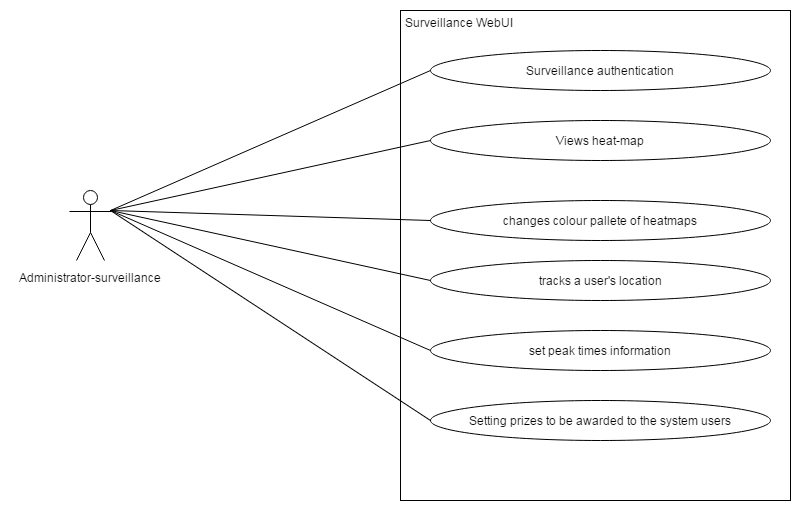
\includegraphics[width=\textwidth]{diagrams/Specific_Requirements/surveillance_webUI.png}
\end{figure}
\mbox{}\\
\bigskip

\FuncReq{Surveillance authentication}
 		{Trivial}
    {Trivial}
    {Trivial}

\FuncReq
    { Views heat-map}
		{The remote repository returns metadata for generating heatmaps in browser}
    {Trivial}
    {Trivial}

\FuncReq{Changes to the colour pallete of heatmaps}
		{Trivial}
    {Trivial}
    {Trivial}
	
\FuncReq{Track a user's location}
		{Surveillance user has to select track user option.
		Surveillance user requires user-name of the user that should be tracked.
		Repository returns current location of user if the user is connected.
		Surveillance can view users current location and see distance traveled by user around the campus.}
    {Trivial}
    {Trivial}
\FuncReq{Analyze certain location and set peak times information}
		{Surveillance user has to select the peak times option.
		Surveillance user submits a request to compare system user location times.
		Surveillance user sets peak times information.
		Surveillance user submits peak times to database.}
    {Trivial}
    {Trivial}
\FuncReq{Setting prizes to be awarded to the system users}
		{Surveillance user has option to view statistical data of the users to select the winner for a specific prize.
		 Surveillance can set a prize for the winner.}
    {Trivial}
    {Trivial}
